\subsection{Point distributions}

In this section, X denotes a manifold of class \(C^{r}\) , and x is a point of X.

13.2.1. Let \(\mathcal{A}\) be the set of pairs \((c, t)\) , where \(c = (\mathrm{U}, \varphi, \mathrm{E})\) is a chart of X centered at \(x\) , and where \(t \in \mathrm{TS}^{(r)}(\mathrm{E})\) . Two elements \(((\mathrm{U}, \varphi, \mathrm{E}), t)\) and \(((\mathrm{U}', \varphi', \mathrm{E}'), t')\) of \(\mathcal{A}\) are said to be equivalent if \(t' = \gamma_*(t)\) , where \(\gamma = \varphi' \circ \varphi^{-1}\) . One thus obtains an equivalence relation on \(\mathcal{A}\) ; an equivalence class for this relation is called a point distribution at \(x\) on X.

Let \(\mathrm{T}_{x}^{(r)}(\mathrm{X})\) be the set of point distributions at x on X. If c is a chart of X centered at x, the map

\[
\theta_ {c} \colon \mathsf {T S} ^ {(r)} (\mathrm{E}) \to \mathbf {T} _ {x} ^ {(r)} (\mathrm{X})
\]

which maps \(t\) to the class of \((c, t)\) , is a bijection. In all that follows, we equip \(\mathrm{T}_{x}^{(r)}(\mathrm{X})\) with the structure of a K-vector space obtained by transporting that of \(\mathrm{TS}^{(r)}(\mathrm{E})\) by \(\theta_{c}\) ; this structure does not depend on the choice of \(c\) . Similarly, if \(k \leqslant r\) , we denote by \(\mathrm{T}_{x}^{(k)}(\mathrm{X})\) and \(\mathrm{T}_{x}^{(k)+}(\mathrm{X})\) the images of \(\mathrm{TS}^{(k)}(\mathrm{E})\) and \(\mathrm{TS}^{(k)+}(\mathrm{E})\) under \(\theta_{c}\) ; they do not depend on the choice of \(c\) . An element of \(\mathrm{T}_{x}^{(r)}(\mathrm{X})\) is said to be of order \(\leqslant k\) if it belongs to \(\mathrm{T}_{x}^{(k)}(\mathrm{X})\) . One has

\[
\mathbf {T} _ {x} ^ {(k)} (\mathbf {X}) = \mathbf {T} _ {x} ^ {(0)} (\mathbf {X}) \oplus \mathbf {T} _ {x} ^ {(k) +} (\mathbf {X}).
\]

There exists one and only one element \(\varepsilon_x\) of \(\mathrm{T}_x^{(0)}(\mathbf{X})\) such that we have \(\theta_c(1) = \varepsilon_x\) for every chart \(c\) of \(\mathbf{X}\) centered at \(x\) . If \(t\) is a point distribution in \(x\) , we call the constant term of \(t\) the element \(\lambda\) of \(\mathbf{K}\) such that \(t - \lambda \varepsilon_x \in \mathrm{T}_x^{(r)+}(\mathbf{X})\) ; we say that \(t\) is without constant term if its constant term is zero.

13.2.2. Let F be a separated polynomial space, and let f be a function of class \(C^{r}\) with values in F, defined on a neighborhood of x. Let t be a point distribution at x on X.

Consider a map \(c = (\mathrm{U}, \varphi, \mathrm{E})\) of X centered at \(x\) , and set \(f_c = f \circ \varphi^{-1}\) and \(t_c = \theta_c^{-1}(t)\) ; the element \(\langle f_c, t_c \rangle\) of F defined in 13.1.3 does not depend on the choice of \(c\) ; we denote it \(\langle f, t \rangle\) . One has \(\varepsilon_x(f) = f(x)\) . \(^{(1)}\) The constant term of \(t\) is \(\langle 1, t \rangle\) .

If \(\mathbf{F}'\) is a separated polynormed space and if \(u: \mathbf{F} \to \mathbf{F}'\) is continuous and linear, we have \(\langle u \circ f, t \rangle = u(\langle f, t \rangle)\) .

Suppose that F is a Banach space, and that t is of order \(\leqslant k\) , with k finite. Let \(j \in \mathrm{J}_{x}^{k}(\mathrm{X}, \mathrm{F})\) , cf. 12.1.2, and let \(f \in j\) . Then \(\langle f, t \rangle\) depends only on the jet j; it is denoted \(\langle j, t \rangle\) . The map from \(\mathrm{T}_{x}^{(k)}(\mathrm{X}) \times \mathrm{J}_{x}^{k}(\mathrm{X}, \mathrm{F})\) to F thus defined is bilinear. When F = K, we have set \(\mathrm{J}_{x}^{k}(\mathrm{X}, \mathrm{F}) = \mathrm{P}_{x}^{k}(\mathrm{X})\) , cf. 12.6.2, and we obtain a bilinear form on \(\mathrm{T}_{x}^{(k)}(\mathrm{X}) \times \mathrm{P}_{x}^{k}(\mathrm{X})\) .

13.2.3. Let \(\varphi: X \to Y\) be a morphism of manifolds of class \(C^r\) and let \(y = \varphi(x)\) . Let \(c = (U, \psi, E)\) be a chart of \(X\) centered at \(x\) and let \(c' = (U', \psi', E')\) be a chart of \(Y\) centered at \(y\) ; let \(\bar{\varphi}\) be the expression of \(\varphi\) in these charts (5.3.2), and let \(\bar{\varphi}_*\) be the corresponding map from \(\mathrm{TS}^{(r)}(E)\) to \(\mathrm{TS}^{(r)}(E')\) , cf. 13.1.4. There exists one and only one linear map, denoted \(\mathrm{T}_x^{(r)}(\varphi)\) or \(\varphi_*\) , from \(\mathrm{T}_x^{(r)}(X)\) to \(\mathrm{T}_y^{(r)}(Y)\) making the diagram commutative

\pandocbounded{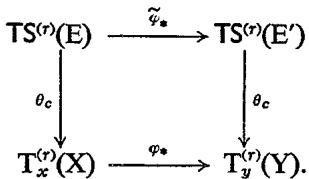
\includegraphics[keepaspectratio]{images/part001_e22e7577.jpg}}

This map does not depend on the choice of \(c\) and \(c'\) . If \(t \in \mathrm{T}_{x}^{(r)}(\mathbf{X})\) , one says that \(\varphi_{*}(t)\) is the image of \(t\) by \(\varphi\) . One has \(\varphi_{*}(\varepsilon_{x}) = \varepsilon_{y}\) . If \(k \leqslant r\) , one has

\[
\varphi_ {*} (\mathrm{T} _ {x} ^ {(k)} (\mathrm{X})) \subset \mathrm{T} _ {y} ^ {(k)} (\mathrm{Y}) \quad \text { and } \quad \varphi_ {*} (\mathrm{T} _ {x} ^ {(k) +} (\mathrm{X})) \subset \mathrm{T} _ {y} ^ {(k) +} (\mathrm{Y}).
\]

If \(\varphi': X \to Y\) is a morphism of class \(C^r\) such that \(\varphi'(x)=y\) , one has \(\varphi_* = \varphi_*'\) if and only if \(j_x^r(\varphi) = j_x^r(\varphi')\) , cf. 12.1.

If \(\varphi\) is an immersion (resp. a submersion) at \(x, \varphi_*\) is injective (resp. surjective); the converse is true if \(\dim_y Y < +\infty\) .

If \(\varphi'\colon\mathbf{Y}\to\mathbf{Z}\) is a morphism of manifolds of class \(\mathbf{C}^{r}\) and if \(t\in\mathbf{T}_{x}^{(r)}(\mathbf{X})\) , one has \((\varphi'\circ\varphi)_{*}(t)=\varphi_{*}^{\prime}(\varphi_{*}(t))\) .

Let F be a separated polynormed space, and let f be a function of class \(C^{r}\) with values in F, defined in a neighborhood of y. We then have

\[
\langle f, \varphi_ {*} (t) \rangle = \langle f \circ \varphi , t \rangle \quad \text {   for   all   } \quad t \in \mathrm{T} _ {x} ^ {(r)} (\mathrm{X}).\tag{1}
\]

For \(t\) given, the relations (1) (for \(f\) and \(F\) variables) characterize \(\varphi_{*}(t)\) ; when \(\dim_y Y < +\infty\) , one may restrict oneself to \(F = K\) .

13.2.4. Suppose that X is an open submanifold of a Banach space E. Denote by \(\varphi_x\) the map \(y \mapsto y - x\) from X into E; the chart \(c = (X, \varphi_x, E)\) is centered at \(x\). We then identify \(\mathrm{T}_x^{(r)}(\mathbf{X})\) with \(\mathrm{TS}^{(r)}(\mathbf{E})\) by means of \(\theta_c^{-1}\). In particular, we have \(\mathrm{T}_x^{(\infty)}(\mathbf{X}) = \mathrm{TS}(\mathbf{E})\) .

Let F be a Banach space, let \(u: E \to F\) a continuous linear map, and let \(x \in E\) , \(y \in F\) such that \(u(x) = y\) . Identify as above \(\mathrm{T}_{x}^{(\infty)}(E)\) with TS(E) and \(\mathrm{T}_{y}^{(\infty)}(F)\) with TS(F). The map

\[
u _ {*} \colon \mathrm{TS(E)} \rightarrow \mathrm{TS(F)} \quad (\text { cf. } 13.2.3)
\]

coincides with the map TS(u) induced by the canonical extension of u to the tensor algebra.

13.2.5. If \(k \leqslant r\) , one denotes by \(\mathrm{T}^{(k)}(\mathrm{X})\) (resp. \(\mathrm{T}^{(k)+}(\mathrm{X})\) ) the set sum of \(\mathrm{T}_a^{(k)}(\mathrm{X})\) (resp. of \(\mathrm{T}_a^{(k)+}(\mathrm{X})\) ) for \(a \in \mathrm{X}\) . A map \(t: \mathrm{X} \to \mathrm{T}^{(k)}(\mathrm{X})\) such that \(t(a) \in \mathrm{T}_a^{(k)}(\mathrm{X})\) for all \(a \in \mathrm{X}\) is called a field of point distributions of order \(\leqslant k\) .

Suppose \(k\) is finite and X is locally of finite dimension. For every \(a \in X\) , the bilinear form \((j, t) \mapsto \langle j, t \rangle\) (cf. 13.2.2) defines an isomorphism \(i_a\) of \(\mathrm{T}_a^{(k)}(\mathrm{X})\) onto the dual \(\mathrm{P}_a^k(\mathrm{X})^*\) of \(\mathrm{P}_a^k(\mathrm{X})\) . The \(i_a\) define a bijection \(i: \mathrm{T}^{(k)}(\mathrm{X}) \to \mathrm{P}^k(\mathrm{X})^*\) , where \(\mathrm{P}^k(\mathrm{X})^*\) denotes the dual of the vector bundle \(\mathrm{P}^k(\mathrm{X})\) ; by transport of structure via \(i^{-1}\) , one endows \(\mathrm{T}^{(k)}(\mathrm{X})\) with a vector bundle structure with base X and class \(\mathbf{C}^{r-k}\) . A field of point distributions of order \(\leqslant k\) is said to be of class \(\mathbf{C}^s\) , with \(s \leqslant r - k\) , if it is a section of class \(\mathbf{C}^s\) of the bundle \(\mathrm{T}^{(k)}(\mathrm{X})\) .

Let \(\varphi\colon\mathbf{X}\to\mathbf{Y}\) be a morphism of manifolds of class \(\mathbf{C}^{r}\) and suppose that Y, like X, is locally finite-dimensional. Then \(\varphi_{*}\colon\mathrm{T}^{(k)}(\mathrm{X})\to\mathrm{T}^{(k)}(\mathrm{Y})\) is a \(\varphi\) -morphism of vector bundles of class \(\mathbf{C}^{r-k}\) .

13.2.6. Let \(k\) be an integer such that \(0 \leqslant k \leqslant r\) . If U is an open set of a finite-dimensional Banach space E, the vector bundle \(\mathbf{T}^{(k)}(\mathbf{U})\) is identified, by virtue of 13.2.4, with the trivial bundle with fibre \(\mathbf{TS}^{(k)}(\mathbf{E})\) .

Take in particular \(E = K^n\) , with \(n \geqslant 0\) , and let \((e_1, \ldots, e_n)\) be the canonical basis of \(E\) . If \(\alpha = (\alpha_1, \ldots, \alpha_n)\) is an element of \(N^n\) , denote by \(\Delta^\alpha\) the element \(\gamma_{\alpha_1}(e_1) \ldots \gamma_{\alpha_n}(e_n)\) of \(TS(E)\) (the product used being the symmetric product of symmetric tensors, cf. A, IV, § 5, no. 3). \(^{(1)}\) The \(\Delta^\alpha\) , for \(|\alpha| \leqslant k\) , form a basis of \(TS^{(k)}(E)\) ; if \(a \in K^n\) , one denotes by \(\Delta_a^\alpha\) the corresponding elements of \(T_a^{(k)}(E)\) . Let F be a separated polynormed space, and f a function of class \(C^r\) , with values in F, defined in a neighbourhood of \(a\) ; if \(\alpha \in N^n\) , the element \(\langle f, \Delta_a^\alpha \rangle\) coincides with the element \((\Delta^\alpha f)(a)\) defined in 2.5.3, 3.2.1 and 4.2.1.

Suppose X is locally finite-dimensional, and let \(\xi = (\xi^1, \ldots, \xi^n)\) be a coordinate system of X in an open set U. If \(a \in \mathbf{U}\) and if \(\alpha\) is a multi-index such that \(|\alpha| \leqslant k\) , one denotes by \((\Delta_{\xi}^{\alpha})_a\) the point distribution at \(a\) whose image under \(\xi\) is the point distribution \(\Delta_{\xi(a)}^{\alpha}\) onto \(\mathbf{K}^n\) ; the distribution fields

\[
\Delta_ {\xi} ^ {\alpha}: a \mapsto (\Delta_ {\xi} ^ {\alpha}) _ {a} \quad (| \alpha | \leqslant k)
\]

form a frame on U of the vector bundle \(\mathbf{T}^{(k)}(\mathbf{X})\) . If \(f\colon \mathbf{U}\to \mathbf{F}\) is of class \(\mathbf{C}^r\) , we set \(\langle f, (\Delta_{\xi}^{\alpha})_a\rangle = \Delta_{\xi}^{\alpha}f(a)\) and denote by \(\Delta_{\xi}^{\alpha}f\) the function \(a\mapsto \Delta_{\xi}^{\alpha}f(a)\) ; it is a function of class \(\mathbf{C}^{r - k}\) in U.

\(^{1}\) If \(m = |\alpha|\) and if \(\Sigma\) is the set of maps \(\sigma\) from \(\{1, \ldots, m\}\) to \(\{1, \ldots, n\}\) such that \(\operatorname{Card}\sigma^{-1}(i)=\alpha_i\), one has

\[
\Delta^ {\alpha} = \gamma_{\alpha_1}(e_1) \dots \gamma_{\alpha_n}(e_n) = \sum_{\sigma \in \Sigma} e_{\sigma(1)} \otimes \dots \otimes e_{\sigma(n)}, \quad \text { cf. A, IV, } \S 5, \text { no. } 4.
\]

